\documentclass[conference]{IEEEtran}
% Packages
%\pdfobjcompresslevel=0
\usepackage{titlesec}
\usepackage{graphicx}
\usepackage[style=numeric, backend=biber, sorting=none,
            url=false, doi=false, isbn=false, eprint=false]{biblatex}
\addbibresource{Communication.bib}
\usepackage{algorithm}
\usepackage{algpseudocode}
\usepackage{booktabs}
\usepackage{float}
\usepackage{multirow}
\usepackage{enumitem}
\setlist[itemize]{leftmargin=*, itemsep=2pt}

% Title page
\title{Swarm Dialogues: Communication policies that shape Embedded Evolution in ESP32 Collectives}
\author{Luis Yallico Ylquimiche}
\date{\today}

\begin{document}

% Title page
\maketitle
%add page numbers
\pagestyle{plain}

% Abstract
\begin{abstract}
We contribute a hardware-in-the-loop swarm that enables peer-to-peer ESP-NOW transmissions and quantifies the impact of communication policies in swarms (3-13 robots). We compare stochastic peer ordering with link-aware scheduling and test two contention controls: per-agent message limits and latency-bounded stochastic delays. Link-aware scheduling lowers latency by 60\%, stochastic ordering spreads information faster but increases collision errors by 72\% at 13 agents across schemes. Bounded micro-delays stabilize latency with minimal throughput cost. Design rule: use stochastic scheduling with micro-delays for rapid diffusion, use link-aware scheduling when latency/jitter robustness is a priority.
\end{abstract}


\section{Introduction}

This study profiles swarm communication on ESP32 hardware and demonstrates how agent density, locomotion, topology inference, imposed message limits, and stochastic transmission policies shape both network quality of service ($QoS$) and embedded evolution performance. Focusing on direct peer-to-peer links, we contribute with an empirical mapping that probes communication bottlenecks flagged in recent surveys, and evidence for extracting tangible design rules for swarm networks. \\

Swarm engineers draw inspiration from social biological systems such as ants, bees or termites to build decentralised robot collectives that are inherently robust to failure, flexible across tasks and scalable in number \cite{hamann_swarm_2018}. In swarm systems, collective intelligence emerges when individual robots trade packets of information among neighbouring robots. Classic ant-colony-optimisation work in the early 2000s has already proven that an indirect information exchange of "virtual-pheromones" can lead to agents collectively discovering optimal routing formations \cite{dorigo_ant_2000}. Hence, communication design is a first-order determinant of emergent behavior in swarms. \\

While coordination and task allocation have been widely studied in swarm robotics, two recent surveys agree that communication bandwidth, latency and energy usage are the main blockers to real-world swarm deployments \cite{ding_advancements_2023}\cite{an_multi-robot_2023}. These issues become more pronounced as swarms sizes scale, resulting in an increase in data volumes being transmitted among peers, often overwhelming individual agents' limited compute capabilities. Beyond sheer capacity, the architecture of the communication also matters. Many swarms rely on blind broadcast communication schemes that scale poorly, with collision rates rising sharply beyond a few dozen peers which tend to reduce the reliability of the network \cite{an_multi-robot_2023}. \\

Communication is equally critical when controllers evolve on-line. Recent embodied evolution studies explain that less communication can enhance swarm performance, as trimming neighbourhood size helps populations forget outdated beliefs and re-adapt faster \cite{hiraga_when_2023}\cite{ding_advancements_2023}. While our context is controller evolution, we instantiate it as a distributed global optimisation problem. Fixing behaviours and evolving solutions to a known objective, isolates the communication effects and makes adaptation dynamics comparable across conditions. \\

To support our investigation, we implement a hardware-in-the-loop framework by leveraging over-the-air (OTA) updates. For embedded evolution we use ESP-NOW with an island-model genetic algorithm (GA). Moving beyond simulation-heavy work, we experiment with Pololu 3Pi+ robots, as shown in Fig. \ref{fig:arena}b, and adopt a state-of-the-art cloud enabled system that captures granular packet and evolution data in real-time, yielding reproducible datasets and enabling controlled parameter sweeps.

\begin{figure}[H]
    \centering
    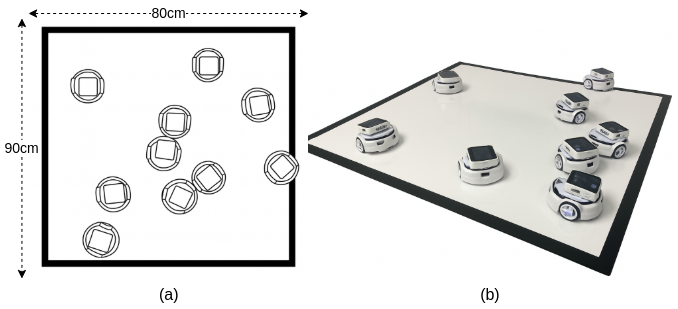
\includegraphics[width=0.49\textwidth]{arena.png}
    \caption{Experimental setup: (a) arena dimensions and (b) example of a Brownian locomotion experiment with 8 robots.}
    \label{fig:arena}
\end{figure}

%might have to explain contention and radio physical properties....

We explore three communication factors and their measurable effects (i) peer ordering, (ii) fixed per-robot message budgets, and (iii) per-packet stochastic transmission delays. We ask, \textbf{RQ1}: whether communication-aware peer ordering using \emph{link-quality} as a lightweight proxy for topology (see Section~\ref{sec:topology-inference}) changes network $QoS$, connection formation patterns, and time-to-consensus relative to stochastic ordering; \textbf{RQ2}: whether these factors influence information diffusion or convergence speed compared with one another; and \textbf{RQ3}: whether micro-delays between transmissions can mitigate collision bursts without harming delivery by measuring proxies such as latency and throughput.

\section{Related Work}
Island-model evolutionary algorithms in \cite{rucinski_impact_2010}, show that migration (genome exchange) topology and connectivity structure govern convergence dynamics not just the migration rate, with the Rastrigin function Eq. \ref{eq:rastrigin}, used to benchmark the performance of different asynchronous evolutionary algorithms. \\

In \cite{hauert_evolved_2009}, controllers are evolved for ad-hoc aerial relays without positional information, using periodic single-hop broadcasts to neighbours. This concept is leveraged on our experimental setting where the agents exploit link-quality proxies to bias their connections. In non-local communication schemes such as \cite{perrin_decentralised_2012}, network-wide epidemic broadcasting known as \emph{flooding} is used to accelerate the diffusion of information, for environmental mapping experiments. In contrast, our study uses \emph{unicast} peer-to-peer links at the data-link layer, enabling direct round-trip time measurements. \\

Constrained connectivity repeatedly appears beneficial. The \emph{"less is more"} effect in \cite{talamali_when_2021}, demonstrates that fewer links and lower swarm densities improve adaptation in swarm consensus tasks, by helping robots discard stale beliefs. A similar effect is also observed by \cite{hiraga_when_2023} over embodied evolution, where limiting the genome-exchange range can support the evolutionary search maintain higher diversity for longer and escape local optima. We explore similar properties which are discussed in Section-\ref{sec:discussion}, the main difference being the data-links used and our message prioritisation algorithm.  \\

Transmission timing also matters. Experiments from \cite{aust_hidden_2022} show that limiting the frequency of communication stabilises swarm behavior, while \cite{tsianos_impact_2012} explains that the speed of consensus among peers tolerates random transmission delays even when agents receive multiple out-of-order messages. Furthermore, non-radio data links have also been explored by \cite{trenkwalder_swarmcom_2020}, which shows that infra-red (IR) line-of-sight local communication can be used in swarms, some benefits include lower energy requirements per bit, moreover we note that IR has limits on bandwidth and bit error probability that scales with range. \\ 

Complementary work by \cite{rabbah_real_2021} examines real-time communication middleware for swarms at the application layer, addressing peer-to-peer IP protocols. In contrast we explore direct peer-to-peer exchange managed without any middleware. \\

% Over-the-air (OTA) mechanisms tailored to swarms have been explored by \cite{varadharajan_over--air_2018}, where updates are distributed as compact patches using gossip-style communication protocols to ensure version uniformity across large robot groups. We adapt this concept in Section-\ref{sec:ota} to support synchronised firmware across our deployment. \\


\section{Experimental Setting}

In this study, we use Eq. \ref{eq:rastrigin} to benchmark the evolutionary performance of the swarm. This global optimisation task was chosen to emulate evolutionary controller optimisation, while no controller was actually evolved the concept of robots sending and receiving genomes from their peers remains the same. Making swarm behaviour a control variable. \\

The environment for the experiments was a rectangular arena measuring 80x90cm without obstacles (Fig. \ref{fig:arena}a), where the initial positions, and number of the robots was determined by the experiment schedule (Table \ref{tab:exp_config}). Across the study, we evaluated swarm under different communication and system configurations. Each experiment manipulates a specific independent variable while holding all other conditions constant. These include:\\

\begin{itemize}
  \item \textbf{Swarm density}: The number of agents deployed simultaneously, ranging from 3 to 13.
  \item \textbf{Locomotion}: Robots were either \emph{stationary} or navigated using a \emph{Brownian motion} gait.
  \item \textbf{Topology inference}: Peer transmission priority was governed by either a \emph{stochastic} shuffle or a \emph{comm-aware} ranking strategy based on link quality metrics.
  \item \textbf{Message limits}: A \emph{message budget} controlled how frequently agents could communicate with one another.
  \item \textbf{Transmission frequency}: Each transmission was optionally delayed by a random interval derived from the maximum observed peer latency.
\end{itemize}

Note that a detailed description of the communication independent variables is available in Section~\ref{sec:comm-layer}.

\subsection{Rastrigin Function}
The Rastrigin function is defined as follows:

\begin{equation}\label{eq:rastrigin}
f_R(\mathbf{x}) = 10n + \sum_{i=1}^{n} \left(x_i^2 - 10\cos(2\pi x_i)\right)
\end{equation}

Where $n$ is the number genes migrating between islands (robots). Whereas, $x$ is the individual genome being evaluated. The function has a global minimum at \( f_R(\mathbf{x}) = 0 \) \cite{rucinski_impact_2010}. Early single-robot trials showed that $n=10$ created enough search difficulty for performance to be measurable across swarm sizes.

\subsection{Robot Platform}\label{sec:robot_platform}
\begin{figure}[h]
    \centering
    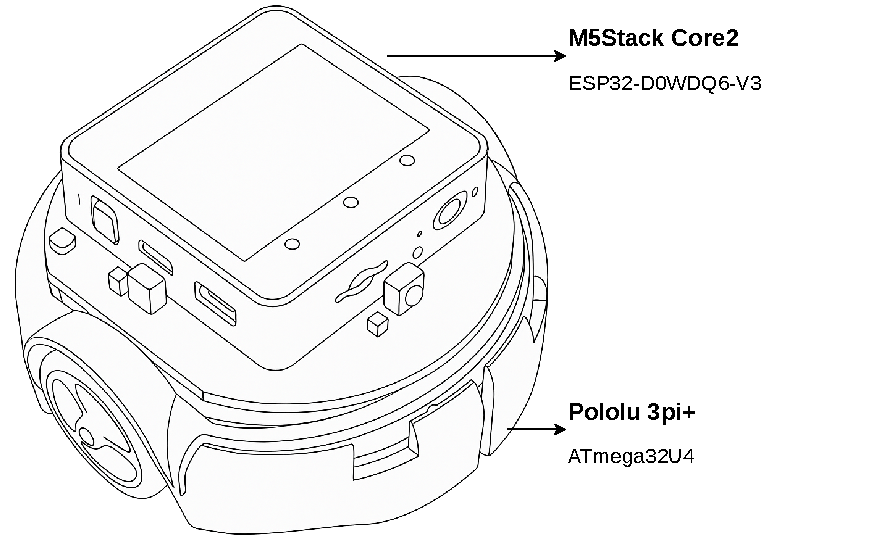
\includegraphics[width=0.45\textwidth]{B2.pdf}
    \caption{The Swarm-B2 platform: M5Stack Core2 and Pololu 3Pi+}
    \label{fig:B2}
\end{figure}

Table~\ref{tab:B2-hardware} summarizes the main hardware components of the Swarm-B2 platform used in this study \cite{odowd_university_2025}. Devices coordinate via an $I^2C$ bus. The ESP32 microcontroller runs dual-core FreeRTOS tasks, that logs real-time data to the local SD card, and manages communication using the ESP-NOW data link (2.4 GHz). \\

\begin{table}[h]
  \centering
  \caption{Swarm-B2 hardware stack}
  \label{tab:B2-hardware}
  \begin{tabular}{p{0.20\linewidth} p{0.18\linewidth} p{0.50\linewidth}}
    \toprule
    Component & Interface & Function \\
    \midrule
    M5Stack Core2 (240 MHz) & $I^2C$ Master       & Embedded evolution, ESP-NOW communication, data logging and user interface \\
    Pololu 3Pi+ (16 MHz)    & $I^2C$ Slave        & Locomotion using bumper and line following sensors \\
    \bottomrule
  \end{tabular}
\end{table}

The Pololu 3Pi+ is equipped with a line following sensor array and two bump sensors, which were used to navigate the around arena as the robots have no positional sensing. A \emph{Brownian-motion} gait was selected to maintain unbiased mobility across the arena and ensure constant movement. The gait code exposes the Pololu 3pi+ slave to the ESP32 master node, this interface lets the ESP32 act as a passenger with override, that can set speed scaling factors or raise \texttt{START}/\texttt{STOP} flags without touching the low-level control loop. Figure~\ref{fig:UI} shows the on-board display, used only for debugging and device status during development. A real-time clock (RTC) synchronised experiment runs across the swarm.

\section{Implementation}\label{sec:implementation}
Reliable and precise data logging is a pre-requisite for evaluating the communication performance and evolution dynamics of the swarm. To achieve this, our framework implements several mechanisms to capture and record key metrics which are explained in this section.

\subsection{System Architecture}\label{sec:architecture}

The firmware was implemented using the Espressif's ESP-IDF framework to provide real-time multitasking. Firmware updates and telemetry data capture are cloud enabled. Code that is written locally in VSCode (ESP-IDF v5.1.4) is rebuilt by GitHub Actions for validation. Only binaries that pass tests are signed and uploaded to an Amazon Web Services (AWS) S3 OTA bucket with a versioned register. On boot, each robot fetches the version register, streams any newer release into an idle OTA slot, and then resets with the latest firmware.

\begin{figure}[hb]
    \centering
    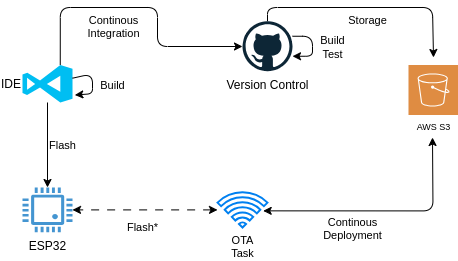
\includegraphics[width=0.45\textwidth]{architecture.png}
    \caption{Integrated architecture: Local development, GitHub repository, AWS S3 storage, and OTA updates.}
    \label{fig:cicd-architecture}
\end{figure}

Experiment schedules ran in batches. During execution, time-stamped messages and event logs are written to a local SD card. After execution, the robot uses WiFi to upload telemetry into an AWS S3 bucket. These files are serialised as JSON, tagged with the \texttt{experiment\_id}, and later processed with AWS Glue/Athena and visualised in PowerBI. This data processing pipeline, allowed us to harvest high-volumes of traceable log data per-robot and per-experiment (see Section~\ref{sec:evaluation-metrics}), while keeping the ESP-NOW data link isolated from Wi-Fi interference during experiments.

% \begin{figure}[H]
%     \centering
%     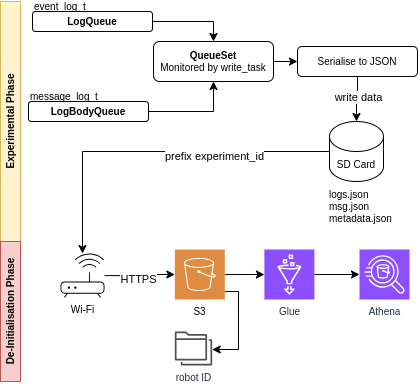
\includegraphics[width=0.45\textwidth]{data_store.png}
%     \caption{Internal data logging pipeline}
%     \label{fig:data-store}
% \end{figure}

\subsection{Embedded Evolution}\label{sec:embedded-evo}

The swarm uses a distributed genetic algorithm \cite{odowd_university_2025}, to find the global minimum for Eq. \ref{eq:rastrigin}. A visual representation of this is shown in Fig. \ref{fig:ga}. As the local population in each agent evolves, the swarm begins to communicate their local fitness and corresponding genome to their peers. \\

\begin{figure*}[t]
    \centering
    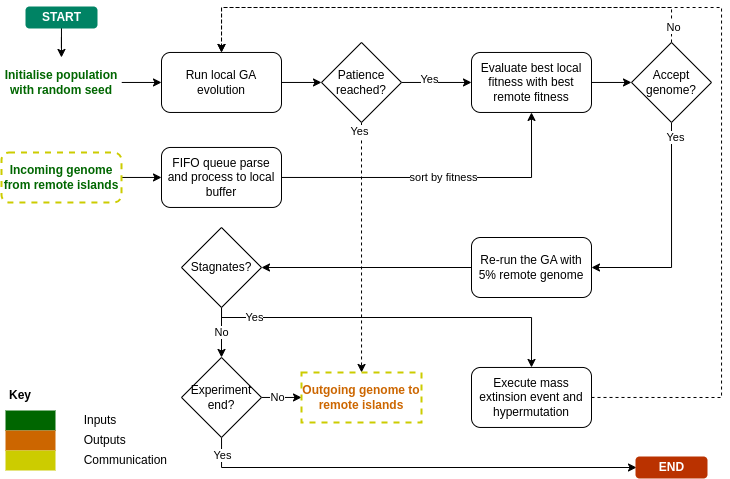
\includegraphics[width=1\textwidth]{ga.png}
    \caption{Distributed island-model GA executed on the ESP32 swarm}
    \label{fig:ga}
\end{figure*}

Our implementation employs an elitist migration strategy, this happens when the local GA reaches a patience threshold and the agent pushes its "best" (lowest fitness score) genome to other swarm members via ESP-NOW. The incoming remote genes from another peer are integrated into the local population by replacing the worst performing $5\%$ individuals, this value was chosen to preserve genomic high fitness locally. \\ 

To avoid stagnation over a local-minima and promote exploration across the swarm, a mass extinction event together with a hyper-mutation mechanism tracks consecutive non-improving generations \cite{krink_self-organized_2001}. In each agent, if the local population's fitness remains stale for over 3 seconds, the mutation probability is temporarily increased and the lowest performing half of the population is re-initialised. \\ 

Evolution continues locally until the experiment ends, triggered either by (i) discovering the global optimum (fitness = 0) or (ii) a 60 s timeout with no convergence. Two FreeRTOS tasks run in parallel, one executes the GA and the other handles ESP-NOW messaging. During shutdown, the \texttt{espnow\_task} flushes any queued packets. Then evolutionary and communication files are uploaded to the telemetry S3 over HTTPS.

\subsection{Message Structure}
We evaluate robot-to-robot communication with a fixed ESP-NOW message schema (Table \ref{tab:out_message}), floats are rounded to $3d.p.$ to send the message in a single transmission. Implications of this design choice are discussed in Section~\ref{sec:discussion}.

\begin{table}[H]
  \centering
  \caption{Message structure used for ESP-NOW fitness value and genome exchange}
  \label{tab:out_message}
  \begin{tabular}{l l p{4cm}}
    \toprule
    \textbf{Field} & \textbf{Type} & \textbf{Description} \\
    \midrule
    \texttt{log\_id} & uint32\_t & Unique internal identifier of the event.\\
    \texttt{robot\_id[5]} & char & MAC identifier for the sender robot plus a null terminator.\\
    \texttt{log\_datetime} & time\_t & Timestamp based on the internal RTC.\\
    \texttt{message[128]} & char & Content of the message including the fitness value and the 10-gene genome delimited by "$|$".\\
    \bottomrule
  \end{tabular}
\end{table}

\subsection{Communication Layer}\label{sec:comm-layer}

In contrast to previous work by \cite{rabbah_real_2021} that explored decentralised communication protocols using middleware, we exploit the ESP32's Medium Access Control (MAC) layer to keep  packet timing and load directly measurable. To do this, we implement ESP-NOW by pre-registering the MAC addresses of all peers in each agent's firmware. We do not view this as a hard scalability limit in the swarm paradigm, as \cite{varadharajan_over--air_2018} explains that gossip-style OTA propagation can disseminate firmware across the swarm, allowing MAC registers to scale without central coordination. \\

Our design uses push only event-driven peer-to-peer messaging, where each device transmits data to peers (migration) without waiting for requests. Using this scheme avoids the complexity of pull-based communication protocols. Incoming messages are handled by a first-in/first-out queue and buffered locally for evaluation. This allowed internal task operations to continue uninterrupted, at the cost of internal memory, from pilot experiments we set the queue size to 40 ($\approx$8KB). \\

Social evidence, in our case is present in the form of the link-quality that arises from migration. Specifically from the latency and Received Signal Strength Indicator (RSSI) that a peer perceives relative to other peers. We use this social evidence to inform our communication strategy and adapt the following policies. \\

\subsubsection{Topology Inference}\label{sec:topology-inference}

We investigate the impact of two communication schemes, based on the social evidence retained locally per-peer. These schemes were designed to influence the priority and order with which each agent sends messages. We use the social evidence as a proxy to infer the topology, under the assumption that distant islands would exhibit different link quality characteristics. These are implemented as follows:

\begin{itemize}
    \item \emph{Stochastic}: Each agent calls a random seed to apply a Fisher-Yates shuffle \cite{fisher_statistical_1963} over the list of peer MAC addresses, sorting them before sending messages to \emph{all peers}. No social evidence bias is used, every order permutation is equally likely.
    \item \emph{Comm-aware}: Each agent ranks its peers based on the most recent measurements of latency and RSSI. Peers with unknown metrics (at initialisation) are prioritised first to ensure social evidence is available. Then, peers are scored by normalizing both latency and RSSI, and those only in the \emph{worst half} (highest latency, lowest RSSI) are messaged.
\end{itemize}

For \emph{stochastic}, the shuffle is defined in Eq.~\ref{eq:fy-shuffle}, where ($j_i$) is a random index drawn from a uniform distribution. $\sigma$ is the random permutation of MAC addresses for each $i$ peer. We can think of this scheme as a \emph{pseudo-broadcast} using unicast communication, as the genome is sent to all peers with negligible delays between transmissions.

\begin{equation}\label{eq:fy-shuffle}
\sigma \;=\; \prod_{i=n}^{2} \bigl(i,\, j_i\bigr), 
\qquad j_i \sim \mathrm{Uniform}\{1,\dots,i\}
\end{equation}

Whereas for \emph{comm-aware}, the scoring for peer $i$ ranking is defined in Eq.~\ref{eq:comm-aware}. Here, the round-trip latency $l$ can be measured via acknowledgements (ACKS). The RSSI $r$ is reported by the ESP-NOW send callback after each successful transmission. If multiple messages have been sent, only the most recent metrics stay in memory. Note that both RSSI and latency are scored equally.

\begin{equation}\label{eq:comm-aware}
Score_i =
\frac{l_i - l_{\min}}{l_{\max} - l_{\min}} +
\frac{r_{\max} - r_i}{r_{\max} - r_{\min}}
\end{equation}

\subsubsection{Message Limits}\label{sec:limited-rate}

Inspired by the reported “less-is-more” effects, we cap the number of migration messages that each robot may broadcast (Eq.~\ref{eq:msg_budget}). Each agent is given a message limit $B$ per sliding time window $W$. Once the limit is exhausted, the robot stays silent until the window advances, no matter how often its onboard genetic algorithm requests migration.  Different from earlier IR-based systems that relied on a short-range \emph{narrowcast} channel \cite{aust_hidden_2022}, we deliver the message to all peers using the topology inference schemes discussed previously.

\begin{equation}\label{eq:msg_budget}
\forall t:\quad M_W(t)=\sum_{i}\mathbf{1}_{\{t-W< t_i \le t\}} \le B
\end{equation}

Here, $t_i$ are the send times, $M_W(t)$ is the number of broadcast messages sent in the last $W=8$s, and the limit is fixed at $B=1$. These values were chosen after pilot tests showed that, without the limit, each peer emitted roughly 15 messages per experiment, effectively limiting migration by half. \\

\subsubsection{Transmission Frequency}\label{sec:transmission-frequency}

To further explore the communication behaviour of the swarm under simultaneous transmission conditions, we modulate the migration interval between islands to spread transmission bursts. Each migration is postponed by random delay drawn from the highest peer-to-peer latency observed so far, which is estimated from the latest ACK round-trip times on every link, described by Eq.~\ref{alg:transmission_freq}:

\begin{equation}\label{alg:transmission_freq}
\Delta t \sim \mathrm{Uniform}\bigl(0,\,L_{\max}\bigr), 
\qquad
L_{\max} = \max_{j}\{\tau_{j}\}
\end{equation}

where ($\tau_{j}$) is the one-hop latency to peer ($j$). If random mode is disabled, ($\Delta t = 0$) and messages are sent immediately by calling \texttt{esp\_now\_send}. The intention of this approach is to control the transmission of messages in a stochastic manner to reduce unintended channel contention in the swarm network.

\subsection{Performance Metrics}\label{sec:evaluation-metrics}

To evaluate the quality of the communication in the swarm, each robot records granular \emph{sender-receiver}: latency $l$ (ms), RSSI $r$ (dBm), net kilobyte rate $t$ (Kbps), transmission-error flags $e$, and per-core CPU load $u$. These raw logs are post-processed by the data pipeline previously detailed in Section \ref{sec:architecture}. AWS then computes the aggregated per-device and per-experiment metrics, (i) $L$ \emph{mean latency}, the time taken for a message to be sent and acknowledged, (ii) $J$ \emph{mean jitter (ms)}, the standard deviation of successive latencies, (iii) $E$ \emph{mean error rate (\%)}, the percentage of messages that were sent but not acknowledged, and (iv) $T$ \emph{mean throughput (Kbps)}, the data is successfully transferred by each agent. To assess overall network performance, a QoS score was computed as:

\begin{equation}
\mathrm{QoS} = w_0 \cdot (1 - \hat{L}) + w_1 \cdot (1 - \hat{J}) + w_2 \cdot (1 - \hat{E}) + w_3 \cdot \hat{T}
\end{equation}

Where, $\hat{L}$, $\hat{J}$, $\hat{E}$, $\hat{T}$ are the normalised global metrics aggregated at the experiment-level in the range of $[0,1]$ and the weights $w_i$ are defined in Table \ref{tab:qos}. A higher QoS value indicates better overall network communication performance. $QoS_c$ weights latency/jitter for consensus/voting tasks, $QoS_s$ weights errors and throughput for sparse deployments. % add performance metrics, adaptation rate is defined as the proportion of agents that share the current lowest fitness score, averaged over 2-second windows.

\begin{table}[H]
\centering
\caption{QoS utility function weights for different swarm robotics applications}
\label{tab:qos}
  \begin{tabular}{@{} lcccc p{3.5cm} @{}}
  \toprule
  \textbf{QoS} & \textbf{$w_0$} & \textbf{$w_1$} & \textbf{$w_2$} & \textbf{$w_3$} & \textbf{Application} \\
  \midrule
  $QoS_c$      & 0.5  & 0.25   & 0.15   & 0.1     & Swarm consensus and voting     \\
  $QoS_s$      & 0.15 & 0.15   & 0.50   & 0.2     & Swarm sparse deployments       \\
  \bottomrule
  \end{tabular}
\end{table}

No inferential statistics were performed. For each condition we executed $n\geq16$ independent runs. Figures report median with IQR (or mean ± SD where noted) across runs. All comparisons are descriptive and should be interpreted accordingly. All experiments used fixed per-run random seeds for GA initialisation. Collected logs and plotting scripts are archived in \cite{yallico_httpsgithubcomyallicorobotics_dissertation_2025}, in the "data\_analysis" folder. \\

\section{Results}\label{sec:results}
As shown in Fig.~\ref{fig:topology}a, the latency and jitter of the swarm network differ significantly between topology inference schemes. Across experiments, \emph{comm-aware} generally achieves lower latency and more stable delivery compared to the \emph{stochastic} mode. Fig.~\ref{fig:topology}b-c show throughput vs topology/message limits. \emph{Stochastic} yields higher raw throughput with wider variability. \\

\begin{figure*}[h]
    \centering
    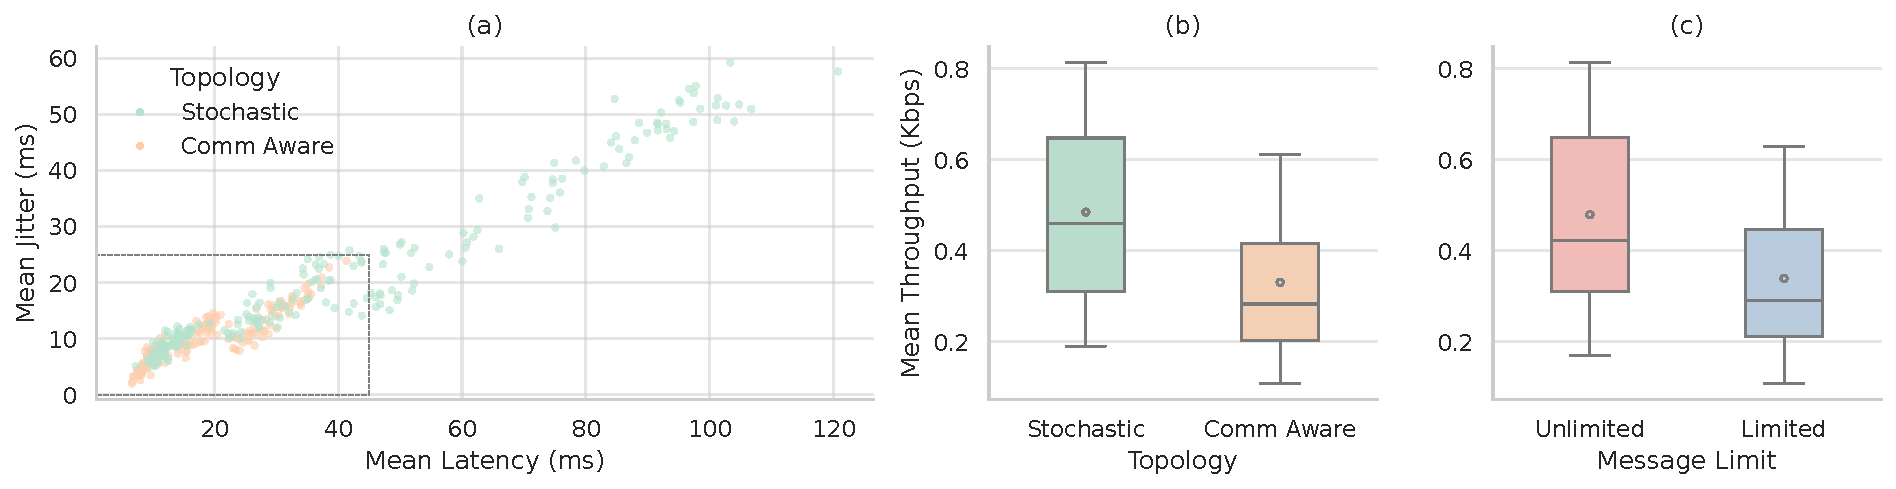
\includegraphics[width=1\textwidth]{topology_impact.pdf}
    \caption{(a) Latency and Jitter relationship under varying topology schemes, (b)(c) throughput distribution under topology and message limit variables}
    \label{fig:topology}
\end{figure*}

Larger swarms reach lower mean fitness scores. \emph{Stochastic} schemes accelerate information diffusion, where $\approx$80\% of agents share the temporal "best" solution 20 seconds earlier than under \emph{comm-aware}. Fig.~\ref{fig:performance}a-b. The degree of connectivity per-peer across time shows that \emph{stochastic} forms more links compared to \emph{comm-aware}, both increasing over time. Fig.~\ref{fig:unique-connections}. \\

\begin{figure*}[h]
    \centering
    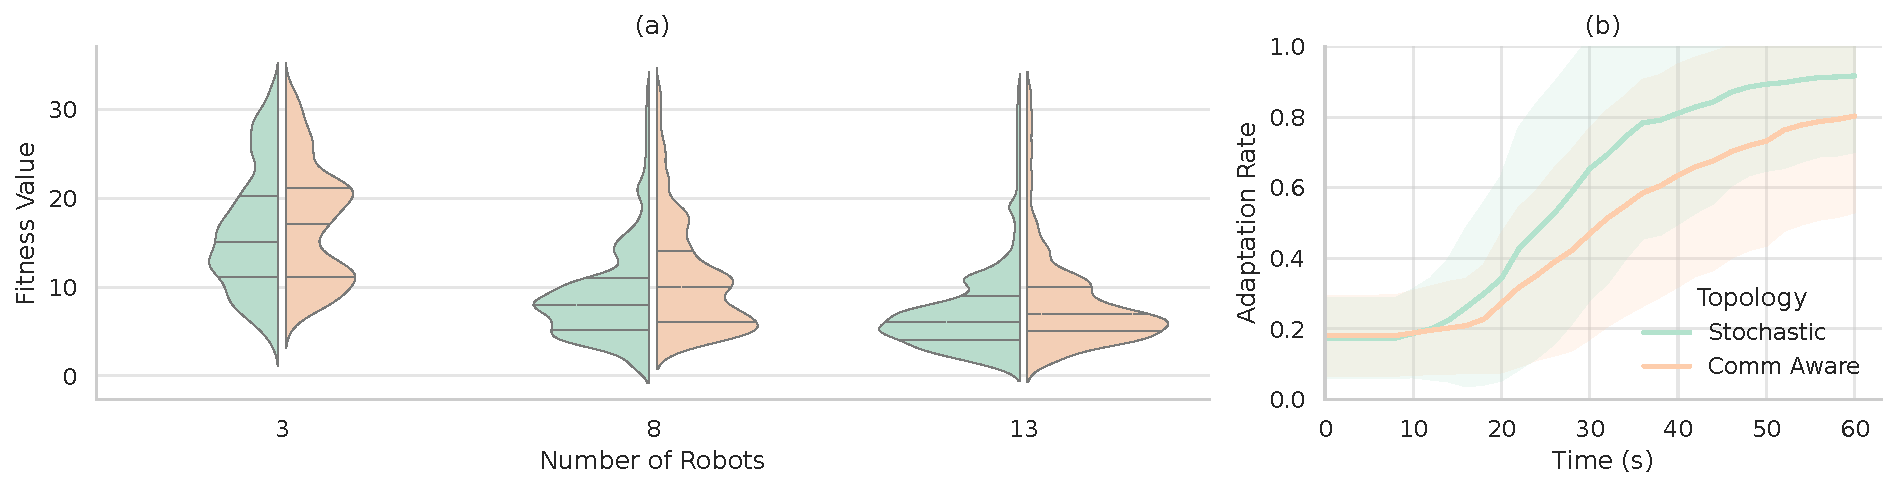
\includegraphics[width=1\textwidth]{performance_impact.pdf}
    \caption{(a) Mean device fitness values across different swarm sizes, (b) mean cumulative percentage of agents converging to the lowest fitness value across $2s$ windows}
    \label{fig:performance}
\end{figure*}

\begin{figure}[h]
    \centering
    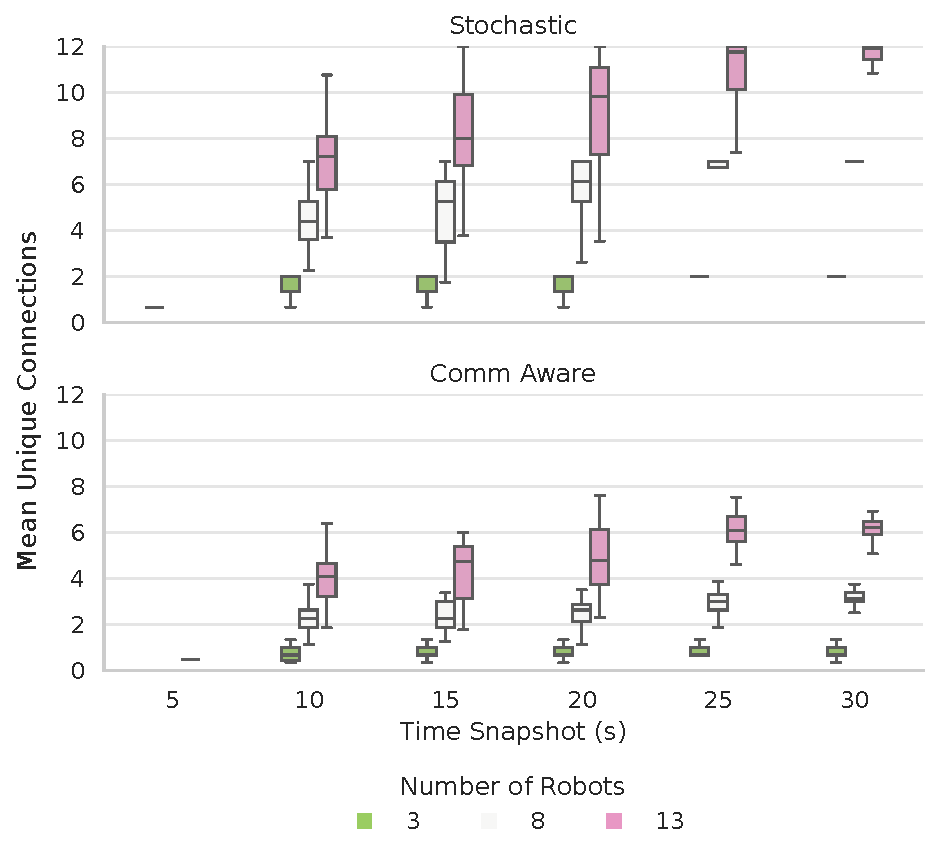
\includegraphics[width=0.46\textwidth]{unique_connections.pdf}
    \caption{Per-peer number of mean connections formed by time snapshot up to 30 seconds for both topology inference schemes}
    \label{fig:unique-connections}
\end{figure}

Error rates are small and comparable for smaller density swarms, rising during 13-agent swarm experiments and when the network operates under the \emph{stochastic} scheme. Fig.~\ref{fig:error-rates}a-b. With regards to locomotion Fig.~\ref{fig:rssi}a shows that Brownian motion results in slightly improved RSSI values, indicating more stable connections compared to static swarms. Whereas \ref{fig:rssi}b suggests no statistical significance between RSSI and topology inference schemes. \\

\begin{figure}[h]
    \centering
    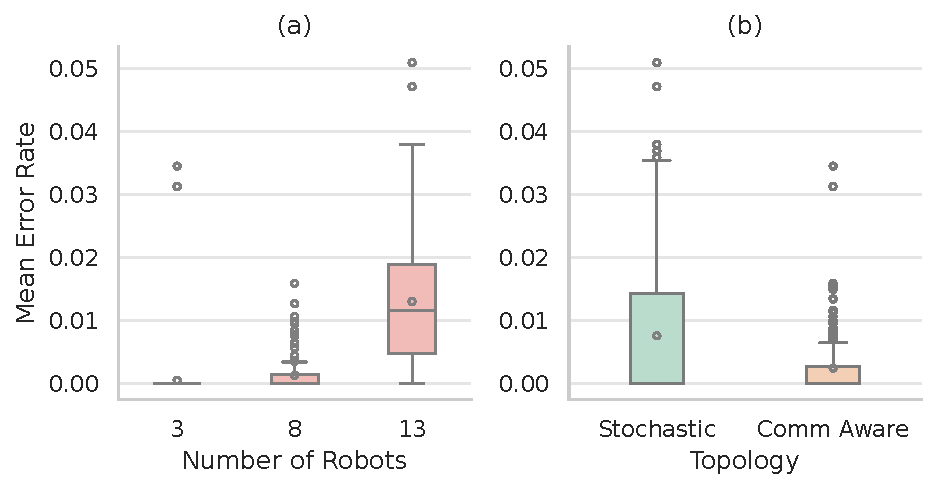
\includegraphics[width=0.47\textwidth]{reliability_impact.pdf}
    \caption{(a) Mean error rates by device across varying swarm sizes, (b) mean error rate for different topology inference schemes}
    \label{fig:error-rates}
\end{figure}

\begin{figure}[h]
    \centering
    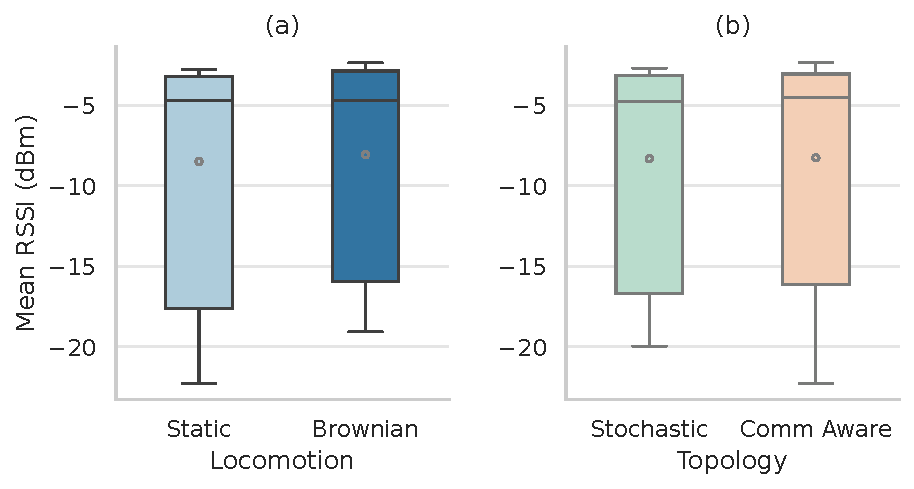
\includegraphics[width=0.47\textwidth]{speed_impact.pdf}
    \caption{(a) Mean RSSI values across different locomotion modes, (b) mean RSSI values across different topology inference schemes}
    \label{fig:rssi}
\end{figure}

Random micro-delays during transmission stabilise latency over time with negligible throughput loss, albeit mean jitter and latency values increase compared to the \emph{comm-aware} scheme (Fig.~\ref{fig:frequency}a-c). The transmissions delays do not block convergence and achieve comparable adaptation rates compared to the \emph{stochastic} scheme (Fig.~\ref{fig:f-performance}a-b). \\

\begin{figure*}[h]
    \centering
    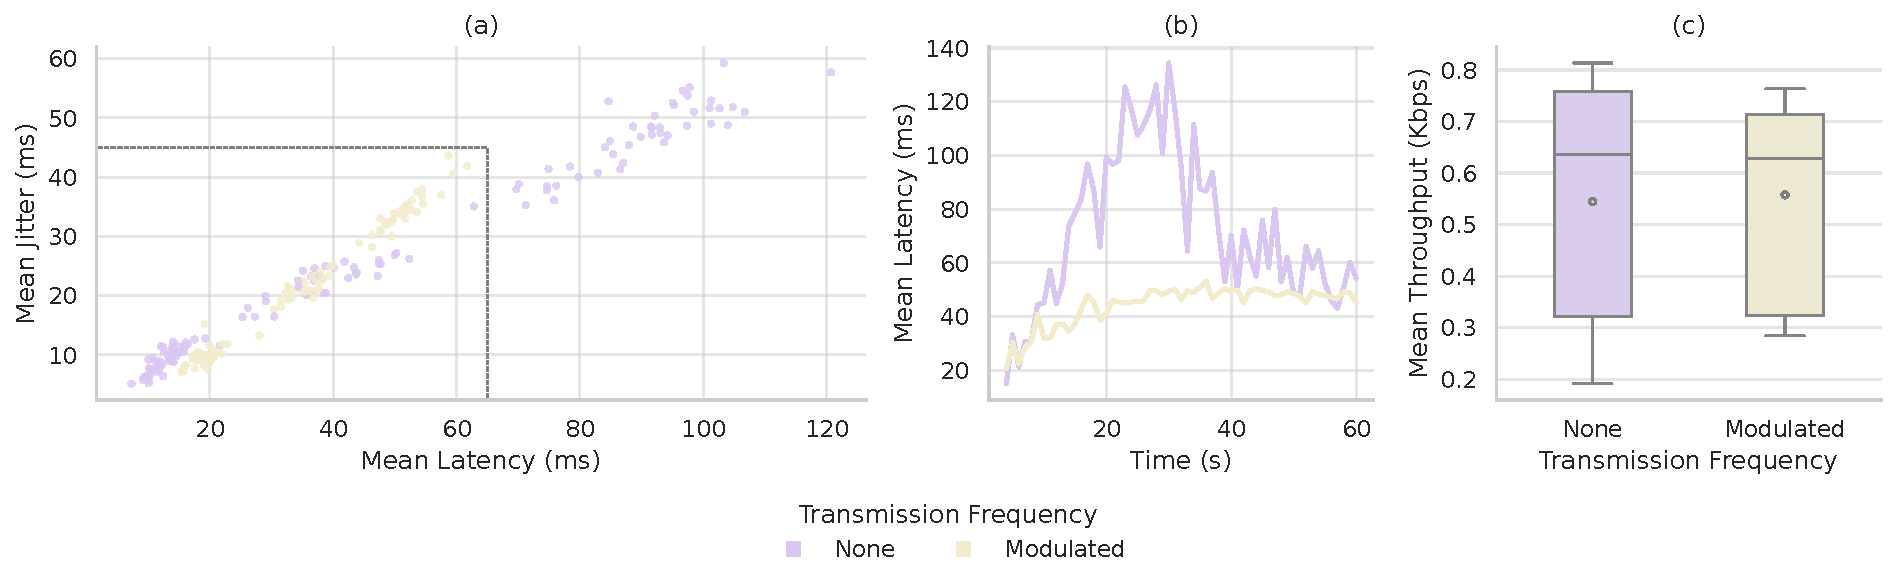
\includegraphics[width=1\textwidth]{frequency_impact.pdf}
    \caption{(a) Latency and Jitter relationship under varying transmission policies, (b) latency across time by transmission setting, (c) throughput distribution by transmission setting}
    \label{fig:frequency}
\end{figure*}

\begin{figure*}[h]
    \centering
    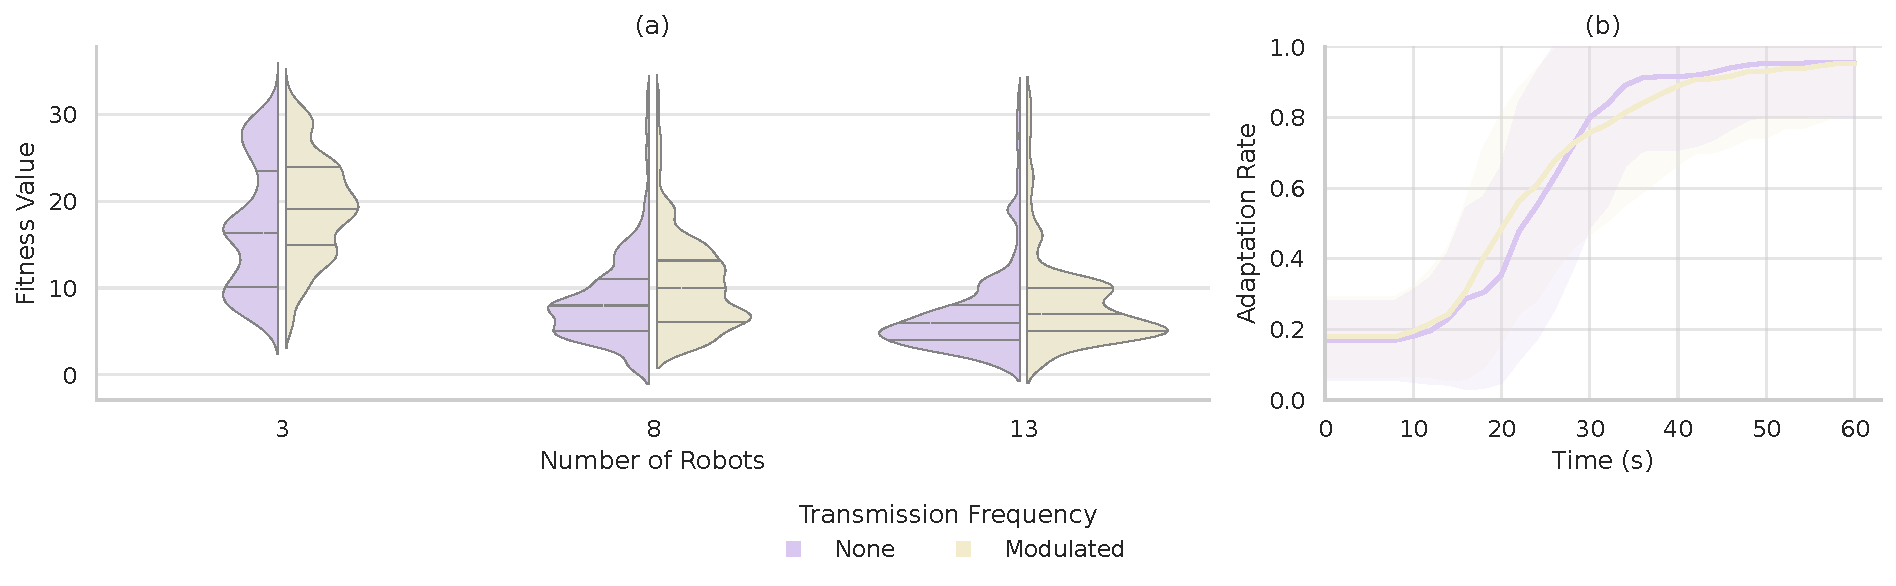
\includegraphics[width=1\textwidth]{f_performance_impact.pdf}
    \caption{(a) Mean device fitness values across different swarm sizes, (b) mean cumulative percentage of agents converging to the lowest fitness value across $2s$ windows}
    \label{fig:f-performance}
\end{figure*}

An evaluation of the characteristics of the $QoS$ metrics for the 13-agent swarm, show that (i) \emph{comm-aware} achieves high $QoS_c$ scores, (ii) modulated transmission shifts toward $QoS_s$ but scores less in $QoS_c$, (iii) message limits do not have a clear effect on QoS, both kernel densities overlap each other. Fig.~\ref{fig:qos}a-d. \\

\begin{figure*}[h]
    \centering
    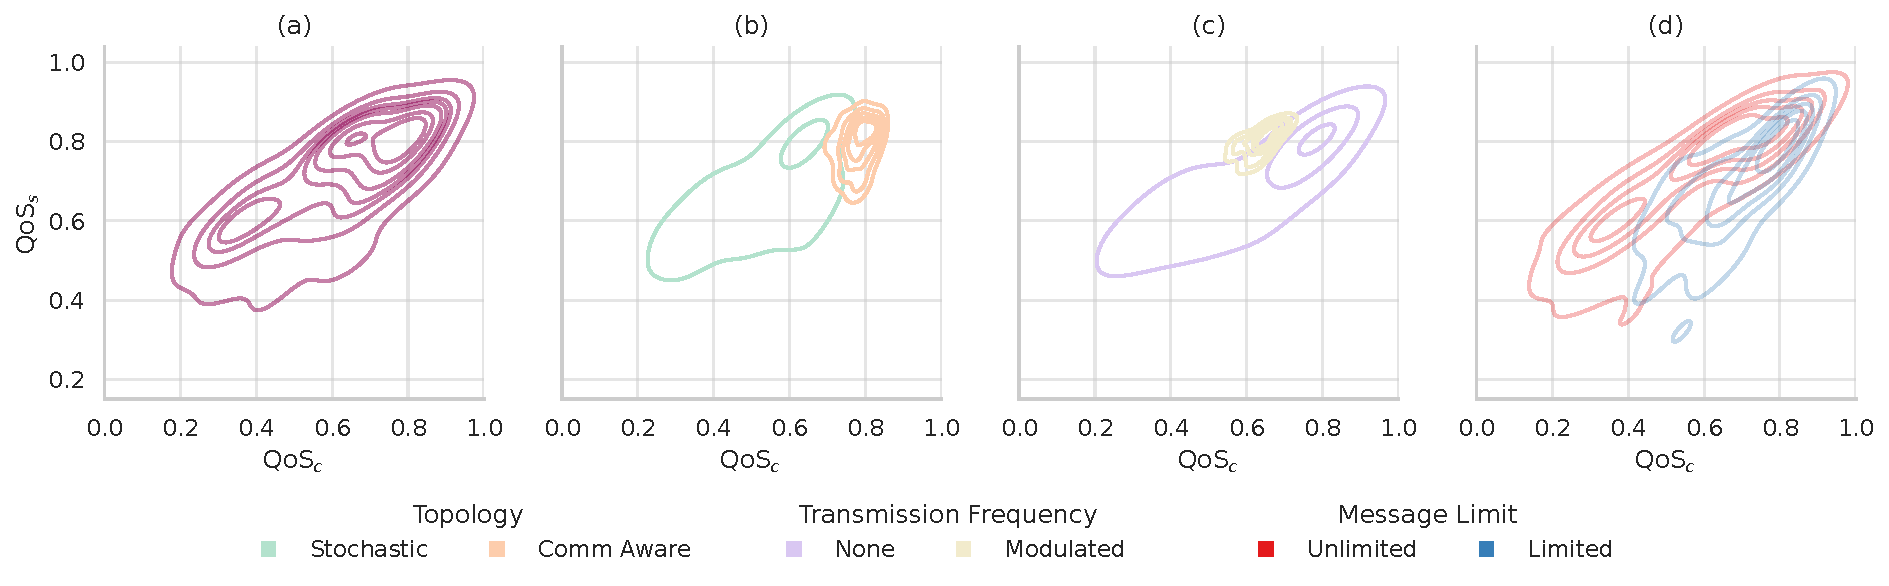
\includegraphics[width=1\textwidth]{qos_impact.pdf}
    \caption{Kernel-density contours showing the joint distribution of two QoS metrics (x: $QoS_c$, y: $QoS_s$) for a 13-agent swarm. (a) pooled across all experimental factors, (b) split by communication topology, (c) split by transmission frequency policy, (d) split by message limit setting}
    \label{fig:qos}
\end{figure*}

\renewcommand{\arraystretch}{0.9}  
\begin{table*}[ht]
\scriptsize
\centering
\caption{Experiment schedule and mean results $\pm~SD$, minimum of 16 runs per-experiment}
\label{tab:exp_config}
\begin{tabular}{c|c|c|c|c|c|c|c|c|c|c}
\toprule
\textbf{Robots} & \textbf{Topology} & \textbf{Locomotion} & \textbf{Message Limit} & \textbf{Transmission} & \textbf{$L$(ms)} & \textbf{$J$(ms)} & \textbf{$E$(\%)} & \textbf{$T$(Kbps)} & \textbf{$QoS_c$} & \textbf{$QoS_s$} \\
\midrule
\multirow{10}{*}{3}
  & \multirow{5}{*}{Stochastic}
    & \multirow{2}{*}{Static}
                 & Unlimited & None      & 15.1$\pm$1.9 & 10.8$\pm$2.1 & 0.0$\pm$0.0 & 0.3$\pm$0.8 & 0.86 & 0.82 \\
  &   &          & Unlimited & Modulated & 20.8$\pm$3.5 & 10.0$\pm$1.8 & 0.1$\pm$0.05 & 0.3$\pm$0.8 & 0.83 & 0.81 \\
  &   &          & Limited   & None      & 12.9$\pm$2.7 & 8.6$\pm$2.4  & 0.0$\pm$0.0 & 0.2$\pm$0.6 & 0.85 & 0.80 \\
  \cmidrule{3-11}
  &   & \multirow{2}{*}{Brownian}
                 & Unlimited & None      & 13.0$\pm$1.8 & 9.3$\pm$1.6 & 0.0$\pm$0.0 & 0.3$\pm$0.8 & 0.87 & 0.83 \\
  &   &          & Unlimited & Modulated & 17.7$\pm$2.9 & 9.5$\pm$2.5 & 0.1$\pm$0.05 & 0.3$\pm$0.8 & 0.84 & 0.82 \\
  &   &          & Limited   & None      & 11.1$\pm$2.3 & 7.3$\pm$2.0 & 0.0$\pm$0.0 & 0.2$\pm$0.6 & 0.87 & 0.81 \\
  \cmidrule{2-11}
  & \multirow{5}{*}{Comm-aware}
    & \multirow{2}{*}{Static}
                 & Unlimited & None      & 11.1$\pm$1.8 & 7.6$\pm$2.7 & 0.0$\pm$0.0 & 0.2$\pm$0.5 & 0.87 & 0.80 \\
  &   &          & Limited   & None      & 10.5$\pm$1.7 & 6.9$\pm$4.0 & 0.0$\pm$0.0 & 0.1$\pm$0.4 & 0.86 & 0.79 \\
  \cmidrule{3-11}
  &   & \multirow{2}{*}{Brownian}
                 & Unlimited & None      & 9.0$\pm$1.6 & 5.9$\pm$2.3 & 0.3$\pm$0.02 & 0.2$\pm$0.5 & 0.87 & 0.77 \\
  &   &          & Limited   & None      & 8.2$\pm$1.7 & 4.5$\pm$2.2 & 0.0$\pm$0.0 & 0.1$\pm$0.3 & 0.88 & 0.79 \\
\midrule
\multirow{10}{*}{8}
  & \multirow{5}{*}{Stochastic}
    & \multirow{2}{*}{Static}
                 & Unlimited & None      & 43.5$\pm$14.6 & 23.7$\pm$4.6 & 0.1$\pm$0.01 & 0.7$\pm$2.6 & 0.72 & 0.84 \\
  &   &          & Unlimited & Modulated & 37.5$\pm$10.4 & 22.2$\pm$7.3 & 0.1$\pm$0.01 & 0.6$\pm$2.5 & 0.75 & 0.84 \\
  &   &          & Limited   & None      & 31.1$\pm$15.2 & 14.7$\pm$5.3 & 0.1$\pm$0.01 & 0.4$\pm$1.8 & 0.78 & 0.82 \\
  \cmidrule{3-11}
  &   & \multirow{2}{*}{Brownian}
                 & Unlimited & None      & 32.7$\pm$13.2 & 20.7$\pm$4.6 & 0.2$\pm$0.01 & 0.6$\pm$2.5 & 0.77 & 0.85 \\
  &   &          & Unlimited & Modulated & 40.0$\pm$9.4  & 21.0$\pm$5.9 & 0.1$\pm$0.01 & 0.6$\pm$2.4 & 0.77 & 0.85 \\
  &   &          & Limited   & None      & 25.6$\pm$13.5 & 12.8$\pm$5.1 & 0.2$\pm$0.01 & 0.4$\pm$1.7 & 0.81 & 0.82 \\
  \cmidrule{2-11}
  & \multirow{5}{*}{Comm-aware}
    & \multirow{2}{*}{Static}
                 & Unlimited & None      & 19.4$\pm$6.3 & 13.3$\pm$3.0 & 0.04$\pm$0.01 & 0.4$\pm$1.2 & 0.84 & 0.84 \\
  &   &          & Limited   & None      & 18.7$\pm$6.7 & 11.3$\pm$3.3 & 0.1$\pm$0.01 & 0.3$\pm$0.9 & 0.83 & 0.80 \\
  \cmidrule{3-11}
  &   & \multirow{2}{*}{Brownian}
                 & Unlimited & None      & 15.3$\pm$5.6 & 10.2$\pm$2.5 & 0.1$\pm$0.01 & 0.4$\pm$1.7 & 0.87 & 0.84 \\
  &   &          & Limited   & None      & 15.0$\pm$6.4 & 8.9$\pm$3.5 & 0.1$\pm$0.02 & 0.3$\pm$0.9 & 0.85 & 0.80 \\
\midrule
\multirow{10}{*}{13}
  & \multirow{5}{*}{Stochastic}
    & \multirow{2}{*}{Static}
                 & Unlimited & None      & 91.5$\pm$33.4 & 47.4$\pm$8.4 & 1.8$\pm$0.7 & 0.77$\pm$3.7 & 0.37 & 0.58 \\
  &   &          & Unlimited & Modulated & 51.2$\pm$20.2 & 33.4$\pm$13.0 & 0.2$\pm$0.1 & 0.72$\pm$3.0 & 0.64 & 0.81 \\
  &   &          & Limited   & None      & 56.0$\pm$33.8 & 22.6$\pm$9.5 & 1.6$\pm$0.5 & 0.58$\pm$2.7 & 0.61 & 0.65 \\
  \cmidrule{3-11}
  &   & \multirow{2}{*}{Brownian}
                 & Unlimited & None      & 86.3$\pm$34.0 & 45.4$\pm$9.2 & 1.9$\pm$0.7 & 0.8$\pm$3.7 & 0.40 & 0.58 \\
  &   &          & Unlimited & Modulated & 51.7$\pm$18.3 & 35.0$\pm$12.8 & 0.3$\pm$0.1 & 0.7$\pm$3.1 & 0.64 & 0.80 \\
  &   &          & Limited   & None      & 53.1$\pm$30.3 & 21.9$\pm$8.3 & 2.4$\pm$0.7 & 0.6$\pm$2.6 & 0.60 & 0.57 \\
  \cmidrule{2-11}
  & \multirow{5}{*}{Comm-aware}
    & \multirow{2}{*}{Static}
                 & Unlimited & None      & 33.5$\pm$16.9 & 17.3$\pm$5.4 & 0.2$\pm$0.02 & 0.6$\pm$2.0 & 0.78 & 0.83 \\
  &   &          & Limited   & None      & 27.5$\pm$16.5 & 11.8$\pm$5.8 & 0.2$\pm$0.01 & 0.4$\pm$1.5 & 0.80 & 0.81 \\
  \cmidrule{3-11}
  &   & \multirow{2}{*}{Brownian}
                 & Unlimited & None      & 31.5$\pm$15.3 & 16.5$\pm$4.1 & 0.7$\pm$0.03 & 0.6$\pm$2.0 & 0.77 & 0.79 \\
  &   &          & Limited   & None      & 26.3$\pm$15.5 & 11.1$\pm$4.7 & 0.8$\pm$0.03 & 0.4$\pm$1.5 & 0.79 & 0.75 \\
\bottomrule
\end{tabular}
\end{table*}


\section{Discussion}\label{sec:discussion}
Across conditions, lower end-to-end latency is driven primarily by limiting concurrent links, not by message limits, achieving sub-50ms comparable to \cite{hauert_evolved_2009} for swarm communication relay scenarios. Under \emph{stochastic} scheduling, pseudo-broadcast rapidly increases unique connections, raising contention. \emph{Comm-aware} limits link formation, avoiding burst traffic and yielding lower median latency and jitter at throughput cost. Time-snapshots of inferred topologies in Fig.~\ref{fig:convergence} illustrate this mechanism, with \emph{stochastic} creating denser transient link sets than \emph{comm-aware} over comparable intervals. In this elitist island-model setup, slower mixing between islands can be useful. Limiting link formation in \emph{comm-aware} reduces premature convergence, allowing for a more diverse genome to persist and be explored longer. This aligns with the observation that overall fitness improves primarily with agent count (Fig. \ref{fig:performance}a), while the fastest adaptation rates arise under the \emph{stochastic} scheme where information diffuses quickly (Fig. \ref{fig:f-performance}b). \\

\begin{figure*}[h]
    \centering
    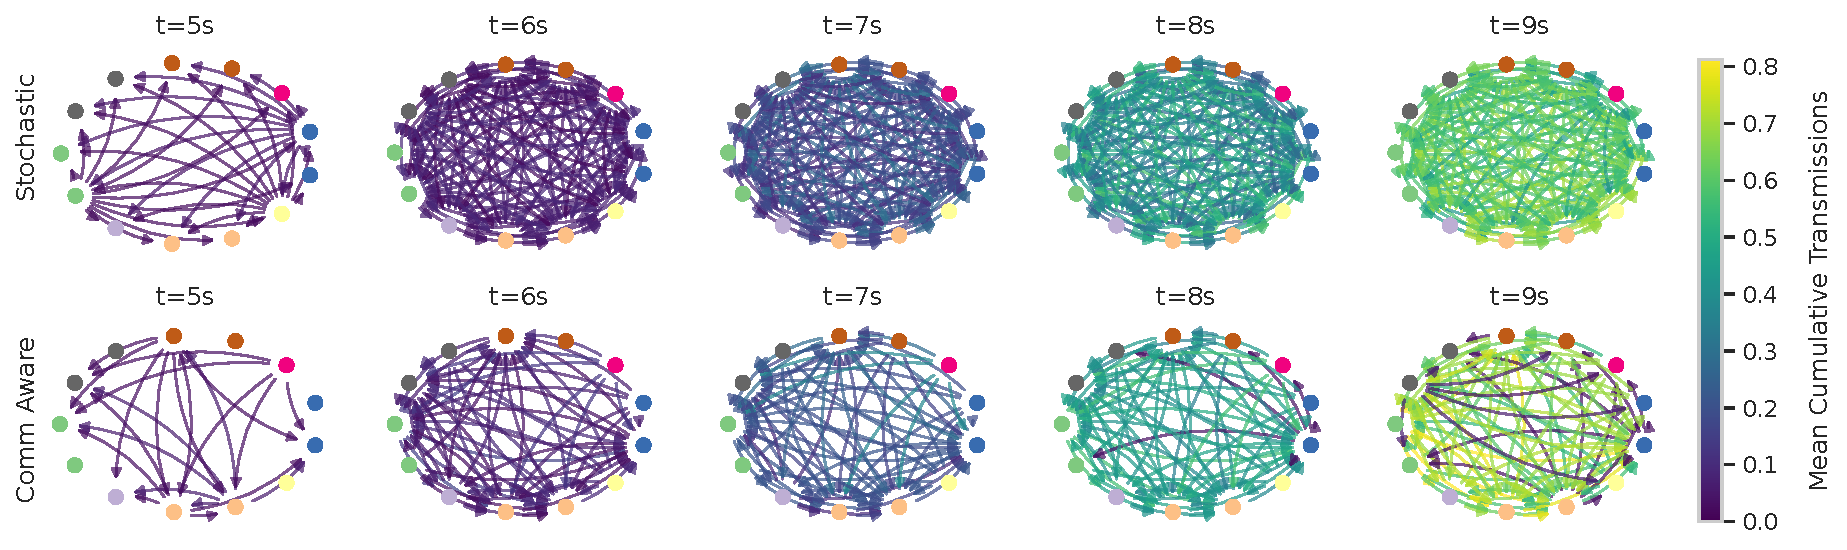
\includegraphics[width=1\textwidth]{convergence_impact.pdf}
    \caption{Temporal snapshots of inferred communication topologies for a 13-agent swarm. Rows: inference scheme, columns: time samples. Nodes are on a fixed circular layout, edges show inferred links and its colour indicates mean cumulative transmissions per node.}
    \label{fig:convergence}
\end{figure*}

\emph{Comm-aware} attains consistently high $QoS$ values by suppressing jitter and keeping low latencies, while \emph{stochastic} achieves higher raw throughput but with higher error rates as agent density grows. Kernel-density plots of $QoS_c$ against $QoS_cs$ in Fig. \ref{fig:qos} show \emph{comm-aware} achieving an overall improved service relative to the overall distribution, whereas frequency modulated \emph{stochastic} shifts the distribution toward $QoS_s$. Message limits show no clear effect. \\

Error rate increases with swarm size, consistent with higher collision probability (Fig. \ref{fig:error-rates}a-b). This effect is independent of locomotion, and becomes most pronounced under \emph{stochastic} at 13-robot swarms. RSSI does not identify topology schemes in this arena, which means that the \emph{comm-aware} scheme is effectively ranking peers by latency. Brownian motion yields slightly lower RSSI than static (Fig.~\ref{fig:rssi}a-b), plausibly by incidental repositioning into stronger links. Verifying this, would require sparser layouts in larger arenas. \\

Introducing frequency modulation under the \emph{stochastic} scheme smooths latency over time (Fig. \ref{fig:frequency}b) without impacting throughput, and preserves fast adaptation rates relative to \emph{comm-aware}. Validating the findings of \cite{tsianos_impact_2012}, the swarm can tolerate transmission delays and attain similar fitness scores compared to having no modulation. For tasks where rapid environmental updates matter such as search and rescue \cite{perrin_decentralised_2012}, this policy provides a low complexity alternative to flooding. \\

Using the fixed genome structure (Table~\ref{tab:out_message}) in a single-channel setup, we observed no detectable effects of mean swarm throughput on GA performance. However, we have not tested whether alternative payload schemas (e.g., partial-genome transfer or non-elitist migration) could change this relationship. The generality beyond the ESP-NOW 250-byte packet limit also remains unverified, larger messages that require fragmentation would likely complicate asynchronous processing, requiring deeper local buffers to avoid packet loss, and also increase compute overhead. \\

Energy consumption matters. Broadcast-heavy policies raise CPU utilisation, whereas link-constraining policies lower processing load (Fig.~\ref{fig:cpu-util}). Energy budgets therefore favour selective link formation and moderated transmissions. For context, ESP-NOW transmit currents are typically an order of magnitude higher than Bluetooth, so depending on the application swarms may need to prioritise partial link formation over fast information diffusion. This trade-off is not abstract, in the author's current role at Unilode Aviation Solutions (the operator of the largest globally distributed aviation IoT network), battery longevity outranks other $QoS$ metrics due to the economics of battery replacement. \\

\begin{figure}[H]
    \centering
    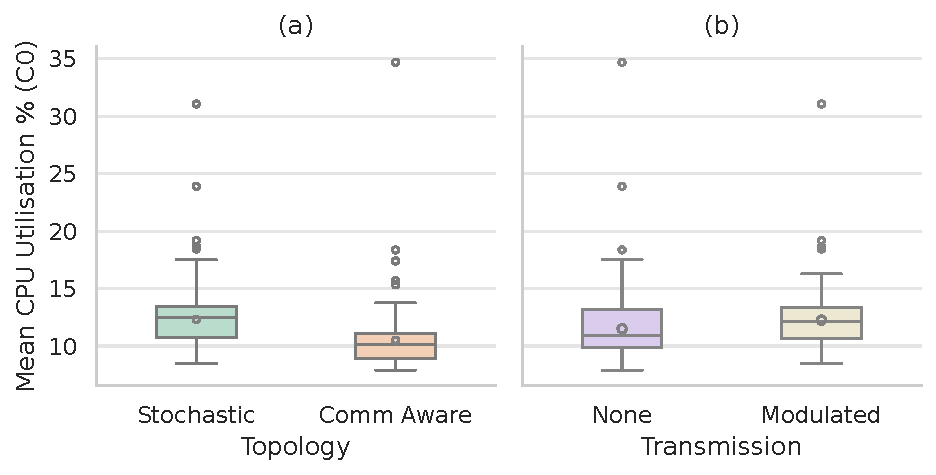
\includegraphics[width=0.46\textwidth]{cpu_util.pdf}
    \caption{Core 0 utilisation by communication policy, excluding message limited experiments}
    \label{fig:cpu-util}
\end{figure}

\emph{Answers to the research questions:} \textbf{RQ1}: Link-aware peer ordering reduces latency and jitter by constraining link formation, at a small throughput cost (Fig.~\ref{fig:topology}a-c; Fig.~\ref{fig:convergence}). \textbf{RQ2}: \emph{Stochastic} ordering accelerates diffusion and earlier convergence, larger swarms achieve lower mean fitness throughout (Fig.~\ref{fig:performance}a-b). \textbf{RQ3}: Latency-bounded random micro-delays smooth latency with negligible throughput loss and preserve adaptation rates (Fig.~\ref{fig:frequency}b-c; Fig.~\ref{fig:f-performance}b).

\subsection{Limitations}

Time resolution is bounded by device RTC drift (roughly $\pm1s$), so message timestamps are only loosely synchronised. Over time results should therefore be interpreted with that tolerance in mind. A second limitation is the environmental variability. Although all trials ran in the same room, they spanned several weeks, and ambient Wi-Fi activity may have varied. We set the ESP-NOW link to channel 6 to avoid nearby access points, but environmental noise cannot be entirely ruled out.

\section{Conclusion}

This work profiled peer-to-peer communication for robot swarms on ESP32 hardware. Across 3 to 13 robot swarms, we found that link formation and transmission timing, drive $QoS$ and adaptation rates on this platform, with throughput volume being secondary. Link formation schemes based on latency social evidence, reduced adaptation rates and information diffusion but did not prevent convergence. Conversely, introducing a small, randomized per-packet transmission delay bounded by the recent peer latency, stabilised network latency without materially impacting throughput.

These findings translate into pragmatic design rules. When rapid network-wide diffusion and high throughput are the priority (e.g., environmental updates or consensus), prioritise stochastic scheduling with randomized transmission micro-delays. When preventing premature convergence and achieving low latencies is of concern, favor limiting effective link formation that will lower contention and support diversity in evolutionary search. This study supports the \emph{“less-is-more"} effects observed in prior swarm studies, where well-scoped constraints can be a feature in decentralized decision making.

\subsection{Future Work}

Future work will stress-test larger and dynamic payloads to probe the limits of our conclusions. We aim to explore how these findings translate to other hardware platforms and combination of protocols, such as IR and Bluetooth. By leveraging the OTA framework, it could also be possible to explore the meta-evolution (e.g., \emph{alpha-evolve}) of the communication policies at the firmware level, enabling task-conditioned tuning for applications in long-term swarm deployments where energy efficiency is critical.

\printbibliography
\section{Appendix}
\begin{figure}[H]
    \centering
    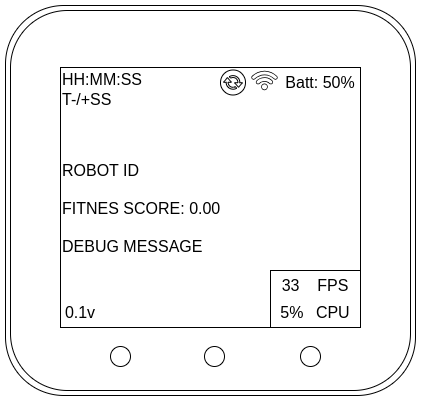
\includegraphics[width=0.35\textwidth]{UI.png}
    \caption{On-board debug/status display}
    \label{fig:UI}
\end{figure}

\end{document}